\documentclass[12pt]{article}
\usepackage{graphicx}
\usepackage{float}

\usepackage[T2A]{fontenc}
\usepackage[utf8]{inputenc}
\usepackage[russian]{babel}

\usepackage{amsmath, amsfonts, amssymb}
\usepackage{amsthm}
% \usepackage{mathpazo}
% \usepackage{fourier}
% \usepackage{newtxmath}
% \usepackage{kpfonts} 

\usepackage[left=2cm, right=2cm, top=2cm, bottom=2cm]{geometry}
\newenvironment{solution}{\begin{proof}[Решение]}{\end{proof}}
\newtheorem*{custom}{}
\newtheorem*{task_1}{Задача 1}
\newtheorem*{task_2}{Задача 2}
\newtheorem*{task_3}{Задача 3}
\newtheorem*{task_4}{Задача 4}
\newtheorem*{task_5}{Задача 5}
\newtheorem*{task_6}{Задача 6}
\newtheorem*{task_7}{Задача 7}

\title{Домашнее задание - 1}
\author{Падалко Александр, Б05-615}

\begin{document}

\maketitle





\begin{task_1}
		
	$T(n) = 3T(\lfloor\sqrt{n}\rfloor) + \log_2{n}$

\end{task_1}

\begin{solution}
		
	Пусть $n = 2^m$, $m = \log_2{n}$, 
	$\sqrt{n} = \frac{m}{2}$

	$T(n) = S(m) = 3S(\frac{m}{2}) + m$

	$S(m)$ можем найти с помощью мастер-теоремы о рекурсии,
	в частности $S(m) = a \cdot S(\frac{m}{b}) + {m^c}$, где $a = 3, b = 2, c = 1$.

	Отсюда следует, что поскольку $\log_{a}{b} = \log_2{3} > 1 = c$, то
	$S(m) = \Theta({m^{\log_2{3}}})$

	Значит $T(n) = S(m) = \Theta(m^{\log_2{3}}) 
	= \Theta(({\log_2{n}}) ^ {\log_2{3}})$

\end{solution}





\begin{task_2}

	$T(n) = 2T(\lceil\frac{n}{2}\rceil) + n\log_2{n}$

\end{task_2}

\begin{solution}

	Рассмотрим, как выглядит $T(n)$ при разделении на уровни.

	В частности, на первом (самом высоком) уровне имеет просто 
	$n \log_2{n}$. Затем $2\cdot\frac{n}{2}(\log_2{\frac{n}{2}}) = 
	n (\log_2{n} - 1)$. На уровне $k$ имеем: $n (\log_2{n} - k)$. Значит,
	по сути, хотим найти $\sum_{0}^{\log_2{n}} n (\log_2{n} - k) = 
	n \cdot \sum_{0}^{\log_2{n}} (\log_2{n} - k) = n \cdot \log_2{n} 
	(\log_2{n} + 1) = \Theta(n \log^2_2{n})$

\end{solution}






\begin{task_3}
	
	$T(n) = \sqrt{n} \cdot T(\lfloor \sqrt{n} \rfloor) + n$

\end{task_3}

\begin{solution}

	Пусть $S(n) = \frac{T(n)}{n}$

	$S(n) = \frac{T(n)}{n} = 
	\frac{T(\lfloor \sqrt{n} \rfloor)}{\sqrt{n}} + 1 = 
	S(\sqrt{n}) + 1$

	Пусть $n = 2^m, m = \log_2{n}, \sqrt{n} = \frac{m}{2}$

	$S(n) = P(m) = P(\frac{m}{2}) + 1 = \Theta({\log_2{m}}) = 
	\Theta({\log_2{\log_2{n}}})$

	$T(n) = S(n) \cdot n = \Theta(n\cdot\log_2{\log_2{n}})$

\end{solution}







\begin{task_4}

	$T(n) = T(f(n)) + T(n - f(n)) + 1 + \log_2{min(f(n), n - f(n))},
	f(n) - $ целое число от $1$ до $n - 1$.

\end{task_4}

\begin{solution}
	
	Рассмотрим случай $n - f(n) = f(n)$, т.е. $f(n) = \frac{n}{2}$.

	Тогда $T(n) = 2\cdot T(\frac{n}{2}) + 1 + \log_2{\frac{n}{2}}
	 = 
	 2\cdot T(\frac{n}{2}) + \log_2{n}$

	Пусть $n = 2^m, m = \log_2{n}$

	$T(n) = S(m) = 2\cdot S(m - 1) + m$

	Разобьём $S$ на $P$ и $L$, где $P(m) = 2 \cdot P(m - 1)$, а 
	$L(m) = 2 \cdot L(m - 1) + m$ (то есть первое это просто степенная,
	а вторая, то сколько накопится лишнего относительно степенной).

	Тогда очевидно, что $P(m) = \Theta{(2^m)}$.

	Поскольку остатков накапливается
	по $m$ с каждого значения, попробуем
	представить $L(m)$, как некоторый многочлен: $L(m) = 
	a_0 \cdot m^0 + a_1 \cdot m^1 + ... + a_k \cdot m^k (a_k \neq 0)$

	$L(m) = 2 \cdot L(m - 1) + m$. Пусть старшая степень больше $1$.

	Коэффициенты при старшей степени с левой и правой сторон должны
	быть равны. Причем c левой стороны коэффициент равен $a_k$, с 
	правой стороны $2a_k$, следовательно $a_k = 0$ (противоречие).

	Значит $L(m) = a_0 + a_1 \cdot m = 2\cdot L(m - 1) + m = 
	2\cdot (a_0 + a_1 \cdot(m - 1)) + m = 2(a_0 - a_1) + 
	(2a_1 + 1) \cdot m \implies 2a_1 + 1 = a_1 \implies a_1 = -1
	\implies 2a_0 + 2 = a_0 \implies a_0 = -2$. Значит $L(m)
	= -m - 2$.

	Значит $S(m) = P(m) + L(m) = \Theta{(2^m)} - m - 2 = \Theta{(2^m)}
	= \Theta{(n)} = T(n)$.

	Докажем, что $T(n) = \Theta(n)$. Для этого нам нужно доказать, что 
	существуют
	$c_1$ и $c_2$ такие, что $c_1n \leq T(n) \leq c_2n$. 

	$T(n) \geq c_1n$, так как по итогу по сути, дерево разбиения
	представляет собой некоторое бинарное дерево с $n$ листами.
	Тогда так как при каждом разбиении добавляется $1$, то
	сумма по всем $(n - 1) = \Theta(n)$.

	Теперь докажем, что $T(n) \leq An - B\log_2{n}$. Рассмотрим по 
	индукции. $T(1)$ - константа, значит найдем такие $A$ и $B$
	(при необходимости потом учтем, чтобы для $T(1)$ ничего не 
	сломалось).

	Пусть $m$ - минимальное из $n$ и $(n - f(n))$.
	Тогда $T(n) = T(m) + T(n - m) + 1 + \log_2{m} \leq
	Am - B\log_2{m} + A(n - m) - B\log_2{(n - m)} + 1 + \log_2{m} = 
	An - B\log_2{m} - B\log_2{(n - m)} + 1 + \log_2{m} = 
	An - (B - 1)\log_2{m} - B\log_2{(n - m)} + 1$.
	
	$n - m > \frac{n}{2} \implies \log_2(n - m) \geq \log_2{n} - 1 
	\implies$.

	$T(n) \leq An - (B - 1)\log_2{m} - B(\log_2{n} - 1) + 1 \leq
	An - B\log_2{n}$.

	Получаем, что $T(n) = \Theta(n)$.

\end{solution}





\begin{task_5}

	Реализовать класс deque с операциями: 
	push\_back, 
	pop\_back, 
	push\_front, 
	pop\_front, 
	operator\texttt{[]}.

	Учетное время всех операций должно быть $\mathcal{O}(1)$.

\end{task_5}

\begin{solution}
	
	Рассмотрим такую структуру: 

	Будем хранить некоторый буфер, условно разделенный на $2$ части.
	А именно - часть для $push$ и часть для $pop$.
	По сути, воспринимаем их как $2$ стека, к которым можно обращаться
	не только к самому верхнему элементу, а любому. 

	Когда приходят операции $push\_back$ и $pop\_back$ мы проделываем их 
	со второй частью, если она не пуста, иначе с первой. Аналогично
	операции $push\_front$ и $pop\_front$ мы проделываем с первой
	частью, если она не пуста, иначе со второй. На самом деле, разделение
	условное, так как, по сути, мы просто храним два индекса в буфере,
	которые считаем началом и концом нашего дека соответственно.

	Если один из концов достигает границы допустимого буфера и требует
	еще расширения (то есть выйти за пределы буфера), то мы выделяем
	новый буфер размера = $4 \cdot $ количество элементов в деке
	(если количество нечетное, то увеличиваем до ближайшего четного).
	
	Далее выделяем первую половину имеющихся элементов и помещаем их в 
	конец области $2$ (на рисунке все области одинакового размера - 
	области нового выделенного буфера), то есть последний элемент
	первый элемент должен быть на последнем индексе в области $2$.
	
	Далее оставшиеся элемента перекидываем в начало области $3$.
	Таким образом получим, что элементы снова представляют собой 
	последоввательный блок, но теперь расположенный в другой области 
	памяти. Новая область памяти в $2$ раза больше старой:

	\begin{figure}[H]
		\centering
		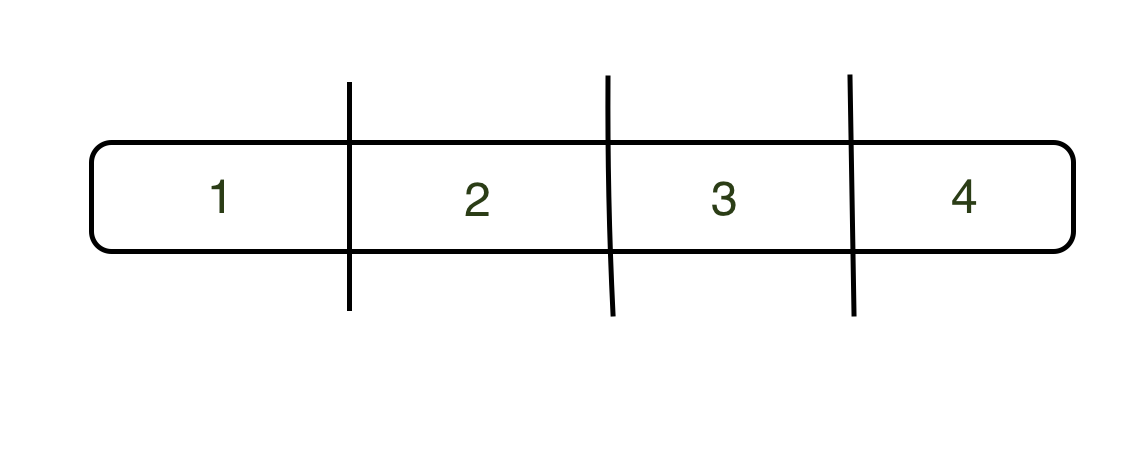
\includegraphics[width=200pt]{deque.png}
		\caption{Части нового буфера}
	\end{figure}

	Теперь проанализируем полученную структуру.

	1) Метод бухгалтерского учета:

	Итак, пусть каждый элемент при добавлении будет иметь $6$ монетки.
	Тогда при обычном $push$ (без расширения) и $pop$ будет тратиться
	одна его монетка. То есть можем отложить еще как минимум $4$ 
	монеты "в копилку" с каждого элемента. 

	Теперь рассмотрим $push$ с раширением. Предполагаем, что выделение
	свободного буфера не тратит времени. Итак, с предыдущего 
	расширения буфера произошло как минимум размер одной четверти буфера
	операций $push$, иначе бы ни один из указателей не дошел бы до
	границы буфера. Имеем, что в таком случае в копилке накоплено
	как минимум $4$ размера одной четверти буфера, то есть размер
	всего буфера. Тогда теперь можем потратить все монетки из 
	"копилки" на перенос всего дека в новый буфер (по $1$ монетке
	на каждый элемент). Получается, что мы никогда не залазим в долги
	по монетам, то есть после любых $k$ операций $\sum_{i = 1}^{k}
	c_i \leq \sum_{i = 1}^{k} c'_i$, где $c_i$ - реальная стоимость
	операции, а $c'_i$ - потраченные монетки.

	Значит после всех $n$ операций мы потратили монеток
	не более $6\cdot n = 
	\Theta(n)$. Таким образом учетная стоимость любой операции 
	$\mathcal{O}(1)$.

\end{solution}

\begin{task_6}

	Дано $5$ камешков и весы. Нужно отсортировать одними сравнениями 
	двух камней и сделать это за минимальное количество взвешиваний.

\end{task_6}

\begin{solution}
	
	Поскольку у нас есть $5! = 120$ исходов и каждое взвешивание
	делит это количество пополам (по сути, идем к листам бинарного
	дерева), то потребуется как минимум $\lceil\log_2{5!}\rceil
	 = \lceil\log_2{120}\rceil = 7$.

	Докажем, что можем сделать это ровно за $7$ взвешиваний. 
	
	Обозначим камешки как $a, b, c, d, e$.

	Взвешивания по порядку:

	$1) a, b$ (Б.О.О. пусть $a < b$)

	$2) c, d$ (Б.О.О. пусть $c < d$)

	$3) b, d$ (Б.О.О. пусть $b < d$)

	\begin{figure}[H]
		\centering
		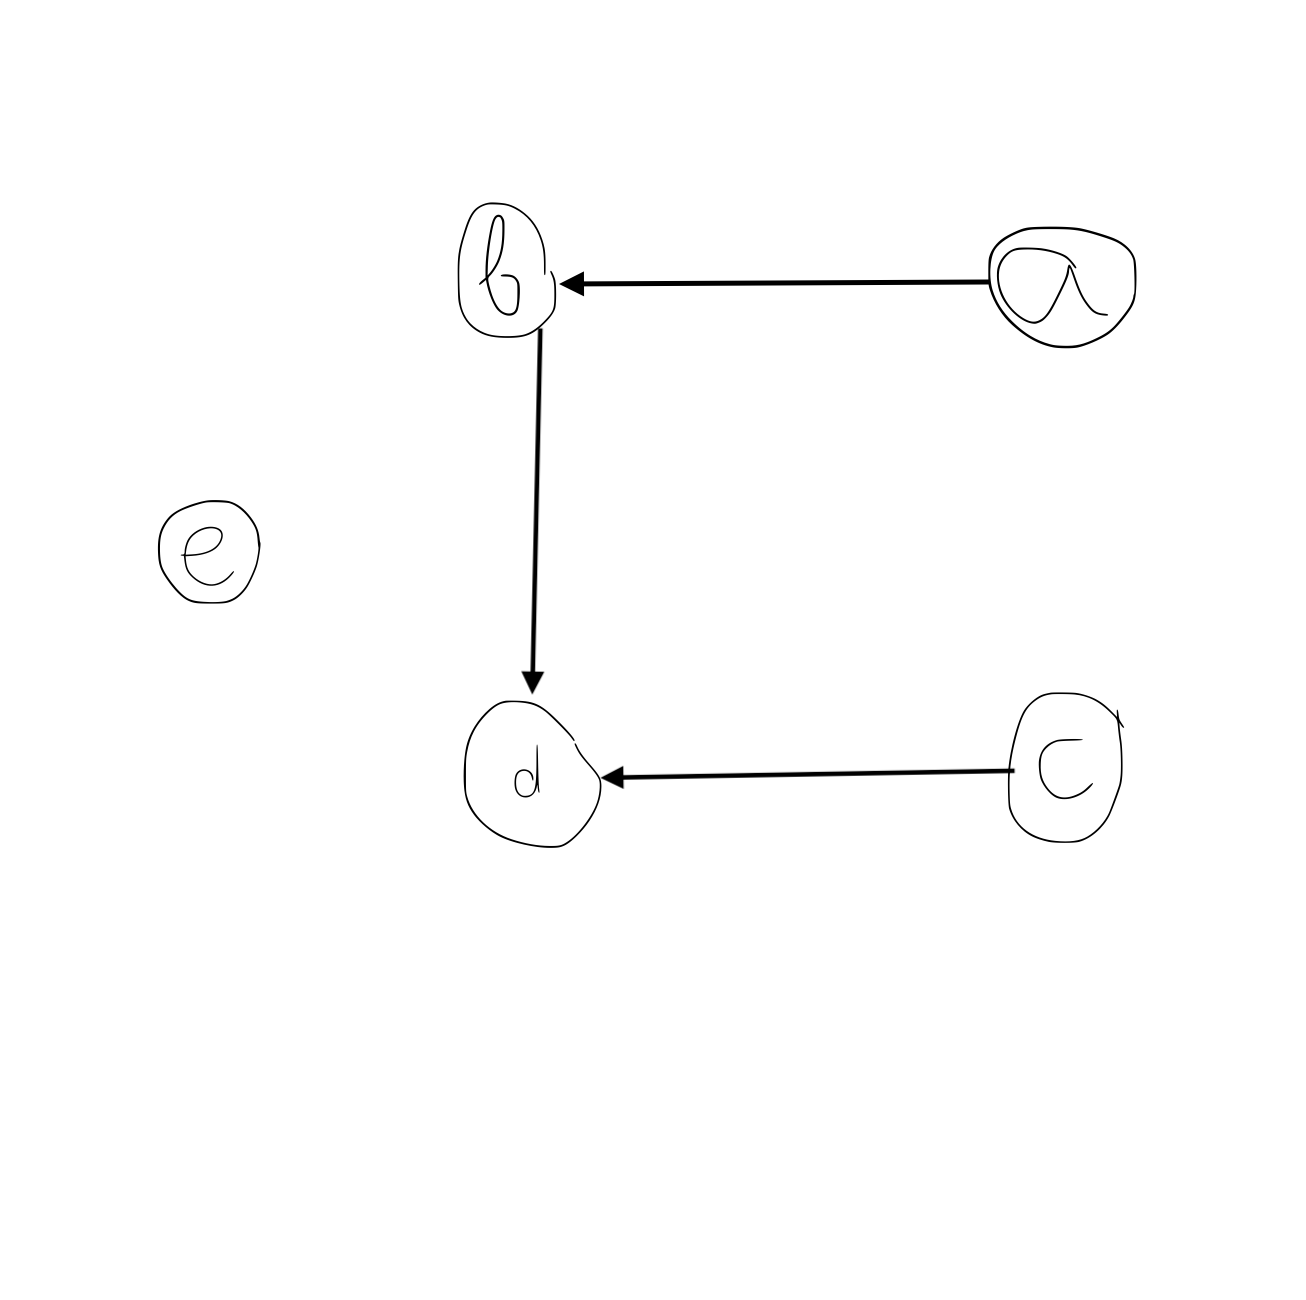
\includegraphics[width=160pt]{3rd.png}
		\caption{После 3-х взвешиваний, стрелка указывает на больший
		из двух камешков (известные на данный момент связи)}
	\end{figure}

	$4) b, e$

	$1$-й случай. Пусть $b < e$, тогда имеем такую картинку:

	\begin{figure}[H]
		\centering
		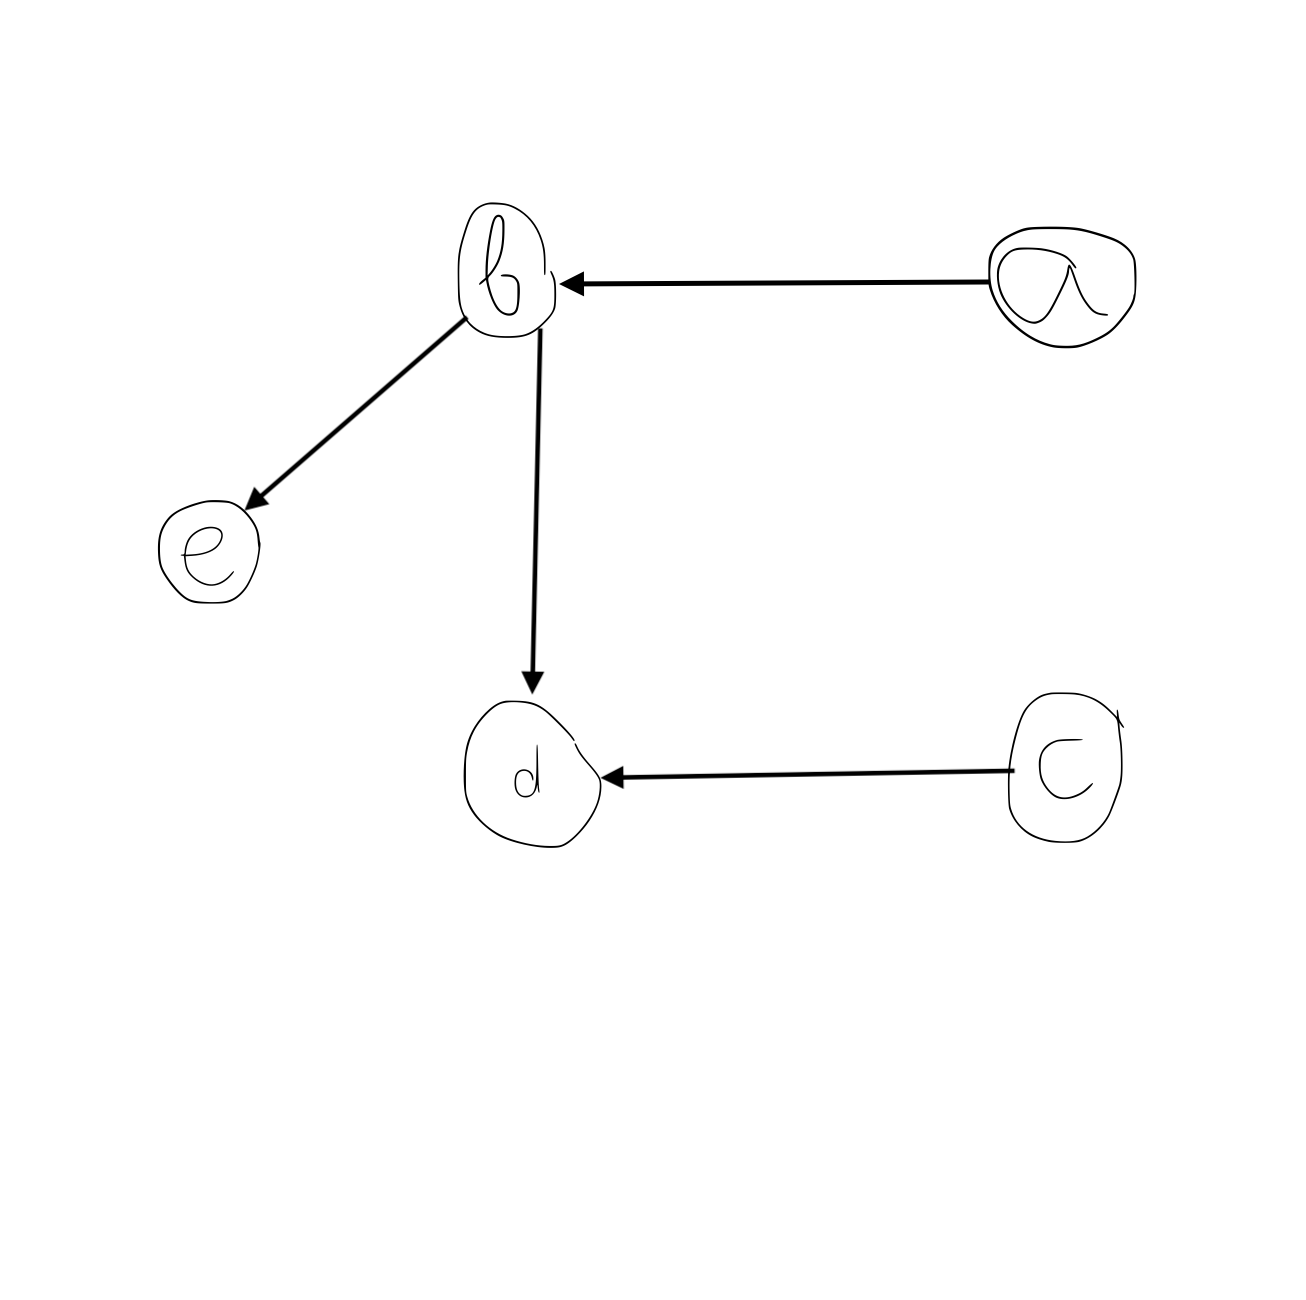
\includegraphics[width=160pt]{be.png}
		\caption{В таком случае нам нужно сравнить $d$ и $e$}
	\end{figure}

	Допустим $d < e$, тогда $e$ наибольший. И у нас еще $2$ взвешивания,
	чтобы определить место $c$ (либо больше $b$, либо от $a$ до $b$,
	либо до $a$; $3$ возможных позиции, значит за $2$ взвешивания
	гарантированно сможем).

	Пусть теперь $d > e$. Теперь сравним $c$ и $b$, и затем сравним
	$c$ либо с $a$, либо с $e$ и тем самым определим итоговый порядок.

	$2$-й случай $e < b$. Сравним теперь $e$ и $a$ и тем самым для
	тройки $a$, $b$, $e$ поймем их окончательный порядок. Затем сравним
	второе число из них с $c$ (это будет большее из $a$ и $e$), и затем
	в зависимости от решения сравним $c$ либо с меньшим из $a$ и $e$,
	либо с $b$.

	Таким образом, за $7$ взвешиваний мы гарантированно найдем порядок
	камешков.

\end{solution}








\begin{task_7}

	Есть $n$ камешков, хотим найти второй минимум. Обозначим
	количество действий, за которое можем сделать это
	за $h(n)$.
	
	Хотим оценить $2^{h(n)}$ асимптотически точно.

\end{task_7}

\begin{solution}

	Для начала заметим, что $h(n) \leq n + \log_2{n} - 2$.

	Чтобы найти за $(n + \log_2{n} - 2)$. По сути построим дерево
	отрезков на минимум на данных нам камешках за $(n - 1)$ взвешивание.
	То есть в листах у нас лежат сами камешки и мы 
	постепенно идем вверх, каждый раз выбирая меньший 
	(более легкий) из камешков. Тогда в корне дерева
	будет находиться минимум. Чтобы теперь найти второй минимум
	посмотрим на путь соединяющий листовой камешек с корнем (длина
	такого пути будет составлять $\log_2 n$ рёбер) и выберем минимальный
	из камешков соседних с путем (то есть по сути, из всех
	камешков, которые из-за минимума отсеялись). Несложно убедиться, 
	что таким образом мы найдем минимум среди оставшихся кроме нашего, 
	то есть, по сути, второй минимум. 
	
	Чтобы выбрать минимум из $\log_2 n$ никак не связанных ранее 
	друг с другом нам достаточно $(\log_2 n - 1)$ взвешиваний.
	Значит всего нам явно достаточно $n + \log_2{n} - 2$ взвешиваний. 

\end{solution}

\end{document}